\documentclass[aps,prapplied,reprint,longbibliography]{revtex4-2}

\usepackage{amsmath,amssymb,amsfonts,amsthm}
\usepackage{graphicx}
\usepackage{booktabs}
\usepackage{xcolor}
\usepackage[hidelinks]{hyperref}

\newtheorem{theorem}{Theorem}
\newtheorem{proposition}{Proposition}

% Generated deterministically by generate_2bga_adv1_assets.py -- do not edit by hand.
\newcommand{\TwoBgaPairsChecked}{6{,}480}
\newcommand{\TwoBgaRankViolations}{0}
\newcommand{\TwoBgaCosetN}{21}
\newcommand{\TwoBgaCosetK}{3}
\newcommand{\TwoBgaGroupsCount}{11}
\newcommand{\TwoBgaParentsCount}{15}
\newcommand{\TwoBgaOddKCount}{16}
\newcommand{\TwoBgaExactCount}{7}
\newcommand{\TwoBgaUpperCount}{9}
\newcommand{\KdSqRatioBest}{3.7895}
\newcommand{\KdSqRatioDFifteen}{3.20}
\newcommand{\KdSqRatioDNine}{3.00}
\newcommand{\KdSqRatioQEight}{3.00}
\newcommand{\KdSqRatioDSeven}{2.6786}
\newcommand{\KdSqRatioFrobTwentyOne}{2.5714}
\newcommand{\KdSqRatioOneEightySix}{2.7258}
\newcommand{\KdSqRatioSFourFive}{1.6667}
\newcommand{\KdSqRatioFrobRankOne}{1.1667}
\newcommand{\TwoBgaOddKRows}{$C_{19} \rtimes C_{3}$ & 57 & $[[114,3,12]]$ & ISD ($\ge 5$) & $(12,12)$ & $(12,6)$ & 3.7895\\
$D_{15}$ & 30 & $[[60,3,8]]$ & ISD ($\ge 5$) & $(8,8)$ & $(8,6)$ & 3.2000\\
$Q_{8}$ & 8 & $[[16,3,4]]$ & Exact & $(4,4)$ & $(6,6)$ & 3.0000\\
$D_{9}$ & 18 & $[[36,3,6]]$ & Exact & $(6,6)$ & $(6,6)$ & 3.0000\\
$C_{31} \rtimes C_{3}$ & 93 & $[[186,3,13]]$ & ISD ($\ge 5$) & $(13,13)$ & $(13,5)$ & 2.7258\\
$D_{7}$ & 14 & $[[28,3,5]]$ & Exact & $(5,5)$ & $(6,6)$ & 2.6786\\
$C_{7} \rtimes C_{3}$ & 21 & $[[42,3,6]]$ & Exact & $(6,6)$ & $(6,6)$ & 2.5714\\
$C_{13} \rtimes C_{3}$ & 39 & $[[78,3,8]]$ & ISD ($\ge 5$) & $(8,8)$ & $(8,6)$ & 2.4615\\
$C_{11} \rtimes C_{5}$ & 55 & $[[110,3,8]]$ & ISD ($\ge 5$) & $(8,10)$ & $(8,6)$ & 1.7455\\
$S_{4}$ & 24 & $[[48,5,4]]$ & Exact & $(4,4)$ & $(6,6)$ & 1.6667\\
$C_{31} \rtimes C_{3}$ & 93 & $[[186,1,17]]$ & ISD ($\ge 5$) & $(17,17)$ & $(17,6)$ & 1.5538\\
$C_{19} \rtimes C_{3}$ & 57 & $[[114,1,13]]$ & ISD ($\ge 5$) & $(13,13)$ & $(13,6)$ & 1.4825\\
$C_{13} \rtimes C_{3}$ & 39 & $[[78,1,10]]$ & ISD ($\ge 5$) & $(11,10)$ & $(10,6)$ & 1.2821\\
$C_{7} \rtimes C_{3}$ & 21 & $[[42,1,7]]$ & Exact & $(8,7)$ & $(7,6)$ & 1.1667\\
$C_{11} \rtimes C_{5}$ & 55 & $[[110,1,11]]$ & ISD ($\ge 5$) & $(13,11)$ & $(11,6)$ & 1.1000\\
$S_{4}$ & 24 & $[[48,3,4]]$ & Exact & $(4,4)$ & $(6,6)$ & 1.0000\\}
\newcommand{\TwoBgaBenchCount}{7}
\newcommand{\TwoBgaMcShots}{800}
\newcommand{\TwoBgaPLow}{0.00079}
\newcommand{\TwoBgaPMid}{0.0020}
\newcommand{\TwoBgaPHigh}{0.0050}
\newcommand{\TwoBgaUnencLow}{0.002368}
\newcommand{\TwoBgaUnencMid}{0.005988}
\newcommand{\TwoBgaUnencHigh}{0.014925}
\newcommand{\BpPhLerFortyTwoHigh}{0.00125}
\newcommand{\BpPhSupprFortyTwoHigh}{11.9}
\newcommand{\BpPhLerDNineAll}{0.0000}
\newcommand{\BpPhLerOneFourteenLow}{0.00125}
\newcommand{\BpPhLerOneFourteenHigh}{0.0075}
\newcommand{\BpCcLerQEightHigh}{0.0025}
\newcommand{\BpCcSupprQEightHigh}{5.97}
\newcommand{\TwoBgaBpOsdRows}{$Q_{8}$ $[[16,3,4]]$ & 0.0000 / 0.00000 & 0.0000 / 0.00000 & 0.0025 / 0.00250\\
$D_{7}$ $[[28,3,5]]$ & 0.0000 / 0.00000 & 0.0000 / 0.00000 & 0.0000 / 0.00250\\
$D_{9}$ $[[36,3,6]]$ & 0.0000 / 0.00000 & 0.0000 / 0.00000 & 0.0000 / 0.00000\\
$C_{7} \rtimes C_{3}$ $[[42,3,6]]$ & 0.0000 / 0.00000 & 0.0000 / 0.00250 & 0.0000 / 0.00125\\
$D_{15}$ $[[60,3,8]]$ & 0.0000 / 0.00000 & 0.0000 / 0.00000 & 0.0000 / 0.00375\\
$C_{19} \rtimes C_{3}$ $[[114,3,12]]$ & 0.0000 / 0.00125 & 0.0000 / 0.00375 & 0.0000 / 0.00750\\
$C_{31} \rtimes C_{3}$ $[[186,3,13]]$ & 0.0000 / 0.00000 & 0.0000 / 0.00250 & 0.0000 / 0.01750\\
\addlinespace
Unencoded $k=3$ baseline $1-(1-p)^3$ & 0.002368 & 0.005988 & 0.014925\\}
\newcommand{\AdvZeroCount}{3}
\newcommand{\AdvZeroRejected}{3}
\newcommand{\AdvOneEvalCount}{5}
\newcommand{\AdvOnePermittedCount}{2}
\newcommand{\AdvConeLimit}{20}
\newcommand{\AdvMinSnr}{10.0}
\newcommand{\AdvChiList}{8, 16, 32, 64, 128}
\newcommand{\AdvWmaxList}{2, 3, 4}
\newcommand{\AdvZeroTwentyEightMpsChiEight}{0.1055}
\newcommand{\AdvZeroTwentyEightMpsChiMax}{0.9805}
\newcommand{\AdvCommMpsChiEight}{0.2852}
\newcommand{\AdvCommPauliWTwoAccPct}{100.0}
\newcommand{\AdvNoMSixPauliWTwoAccPct}{64.3}
\newcommand{\AdvNoMSixPauliWThreeAccPct}{100.0}
\newcommand{\AdvNoMSixPauliWThreeMeanZ}{0.8235}
\newcommand{\AdvEighteenExactPeak}{0.4371}
\newcommand{\AdvEighteenMpsChiMax}{0.1875}
\newcommand{\AdvTwentyFourCz}{372}
\newcommand{\AdvTwentyFourOneQ}{892}
\newcommand{\AdvTwentyFourMirrorOv}{0.3162}
\newcommand{\AdvTwentyFourPauliAccPct}{41.7}
\newcommand{\AdvTwentyFourDroppedLTwo}{0.9998}
\newcommand{\AdvTwentyFourHeliosPeak}{0.3908}
\newcommand{\AdvTwentyFourHqc}{975.4}
\newcommand{\AdvThirtyCz}{465}
\newcommand{\AdvThirtyOneQ}{1{,}115}
\newcommand{\AdvThirtyMirrorOv}{0.2880}
\newcommand{\AdvThirtyPauliAccPct}{46.7}
\newcommand{\AdvThirtyDroppedLTwo}{0.9996}
\newcommand{\AdvThirtyHeliosPeak}{0.3508}
\newcommand{\AdvThirtyHqc}{1{,}218}
\newcommand{\AdvThirtyHqcExact}{1218.0}
\newcommand{\AdvOnePregateRows}{\texttt{adv0\_ctrl\_n12\_d4} & 12 & 32 & Artifact & Win (1.000) & Win (100.0\%) & Win (10) & 0.959 / 121.4 & REJECTED\\
\texttt{adv0\_ctrl\_n20\_d6} & 20 & 76 & Artifact & Win (1.000) & Win (100.0\%) & Win (16) & 0.914 / 261.8 & REJECTED\\
\texttt{adv0\_ctrl\_n28\_d8} & 28 & 158 & Artifact & Win (0.980) & Fail (96.4\%) & Fail (28) & 0.841 / 510.6 & REJECTED\\
\addlinespace
\texttt{adv1\_commuting\_phase\_n24\_L3} & 24 & 192 & No (0.12) & Win (0.188) & Win (100.0\%) & Fail (24) & 0.285 / 518.4 & REJECTED\\
\texttt{adv1\_chorded\_2q\_n28\_L5\_no\_m6} & 28 & 364 & No (0.32) & Fail (0.000) & Win (100.0\%) & Fail (28) & 0.364 / 985.0 & REJECTED\\
\texttt{adv1\_chorded\_m6\_n18\_L4\_small\_cone} & 18 & 243 & No (0.35) & Win (0.188) & Fail (55.6\%) & Win (18) & 0.348 / 644.6 & REJECTED\\
\texttt{adv1\_chorded\_m6\_n24\_L5} & 24 & 372 & No (0.32) & Fail (0.000) & Fail (41.7\%) & Fail (24) & 0.391 / 975.4 & \textbf{PERMITTED}\\
\texttt{adv1\_chorded\_m6\_n30\_L5} & 30 & 465 & No (0.29) & Fail (0.000) & Fail (46.7\%) & Fail (30) & 0.351 / 1218.0 & \textbf{PERMITTED}\\}


\begin{document}

\title{Left-Right Rank Duality in Non-Abelian Two-Block Group-Algebra Quantum LDPC Codes and a Three-Attack Classical-Hardness Pre-Gate for Looped Non-Mirror Peaked Circuits}

\author{Devin Phillip Davis}
\affiliation{Agile Defense Systems LLC}

\date{November 23, 2026}

\begin{abstract}
All-to-all quantum charge-coupled device (QCCD) trapped-ion processors unlock both non-planar quantum low-density parity-check (qLDPC) memory codes and long-range chorded circuits whose output peaks resist polynomial-time classical algorithms. Here we establish rigorous algebraic and computational results across both domains in verified \texttt{SIMULATED} benchmarks (\texttt{provider\_job\_id: null}) calibrated to the 98-qubit Quantinuum \texttt{Helios-1} architecture. First, for Lin--Pryadko two-block group-algebra (\texttt{2BGA}) Calderbank--Shor--Steane (CSS) codes $H_X = [L(a)\mid R(b)]$, $H_Z = [R(b)^\top \mid L(a)^\top]$ over $\mathbb{F}_2[G]$, we prove via the group-inversion anti-automorphism and Frobenius / Wedderburn--Artin duality that $\mathrm{rank}_{\mathbb{F}_2}(H_X) = \mathrm{rank}_{\mathbb{F}_2}(H_Z)$ holds identically for every finite group $G$---including odd-order non-abelian Frobenius metacyclic groups $C_p \rtimes C_q$---forcing unquotiented regular \texttt{2BGA} codes to carry strictly even logical dimension $k = 2(|G| - \mathrm{rank}_{\mathbb{F}_2}(H_X))$, verified with \TwoBgaRankViolations{} violations across \TwoBgaPairsChecked{} subset pairs over \TwoBgaGroupsCount{} non-abelian groups. Breaking left-right duality via subgroup-quotient coset \texttt{2BGA} (exemplified by a $D_9/\mathbb{Z}_2$ code with $n=\TwoBgaCosetN{}, k=\TwoBgaCosetK{}$) or symplectic minimum-weight logical gauge pinning yields \TwoBgaOddKCount{} odd-$k$ ($k \in \{1, 3, 5\}$, $d \ge 4$) non-abelian CSS codes, including exact-distance $D_9$ $[[36,3,6]]$ ($kd^2/n = \KdSqRatioDNine{}$), $C_7 \rtimes C_3$ $[[42,3,6]]$ ($\KdSqRatioFrobTwentyOne{}$), and ISD-witnessed $C_{19} \rtimes C_3$ $[[114,3,12]]$ ($\KdSqRatioBest{}$), achieving strong logical suppression under Sum-Product \texttt{BP+OSD-CS} decoding. Second, because prior twirled-mirror \texttt{ADV-0} peaked circuits fail classical-hardness audits due to hidden $U^\dagger U$ cancellation, we introduce the fail-closed \texttt{ADV-1} pre-gate requiring every candidate to defeat bounded-$\chi$ matrix-product-state ($\chi \le 128$), truncated Pauli-path ($w_{\max} \le 4$), and causal light-cone ($|C| \le \AdvConeLimit{}$) attacks prior to QPU allocation. While naive non-mirror chorded circuits without Pauli amplification fail at $w_{\max}=3$ ($\AdvNoMSixPauliWThreeAccPct{}\%$ secret recovery), appending the 15-\texttt{CX} involution $M_6 = J_6 - I_6 \pmod 2$ lifts every single-qubit output $Z_j$ to exact Pauli weight five, enabling 24-qubit and 30-qubit chorded circuits to survive all three attacks with predicted \texttt{Helios-1} peak probabilities $\AdvTwentyFourHeliosPeak{}$ and $\AdvThirtyHeliosPeak{}$.
\end{abstract}

\maketitle

\section{Introduction: Fault-Tolerant Memory and Pre-Submission Hardness Gating on All-to-All QCCD Architectures}
\label{sec:intro}

Reconfigurable trapped-ion quantum charge-coupled device (QCCD) architectures such as Quantinuum \texttt{H2-1} and 98-qubit \texttt{Helios-1} support arbitrary nonlocal two-qubit connectivity via physical ion transport without SWAP-routing overhead~\cite{moses2023race}. Nonlocal connectivity transforms two central problems in near-term fault tolerance and verifiable quantum benchmarking: first, high-rate quantum low-density parity-check (qLDPC) codes are no longer restricted to planar Euclidean lattices~\cite{breuckmann2021quantum,panteleev2022asymptotically,bravyi2024high}; second, native long-range chords allow compact circuit families with maximal bipartite entanglement growth and full-register causal light cones~\cite{aaronson2025verifiable,gharibian2025peaked}.

Despite this architectural synergy, both problems confront sharp structural pitfalls when designs are extrapolated heuristically. On the coding side, abelian bivariate-bicycle codes over $\mathbb{Z}_\ell \times \mathbb{Z}_m$ predominantly encode even numbers of logical qubits ($k$ even), motivating searches over non-abelian finite groups $G$ whose group algebras $\mathbb{F}_2[G]$ decompose via Wedderburn--Artin theory into non-commutative matrix rings $M_q(\mathbb{F}_{2^f})$~\cite{lin2024quantum,kovalev2013quantum}. A natural hypothesis is that replacing abelian groups with odd-order non-abelian Frobenius groups $C_p \rtimes C_q$ in the standard two-block group-algebra (\texttt{2BGA}) construction might directly break $X$/$Z$ rank symmetry and yield odd logical dimensions $k$ (such as $k=1$ or $k=3$ for modular three-logical-qubit fault-tolerant gadgets). In Sec.~\ref{sec:duality}, we prove that this naive hypothesis fails identically: Frobenius trace and inversion anti-automorphism duality lock $\mathrm{rank}_{\mathbb{F}_2}(H_X) = \mathrm{rank}_{\mathbb{F}_2}(H_Z)$ across every finite group $G$. In Sec.~\ref{sec:oddk}, we show how breaking left-right regularity---either algebraically via subgroup-quotient cosets $G/H$ or symplectically via minimum-weight logical gauge pinning---constructively unlocks \TwoBgaOddKCount{} odd-$k$ non-abelian CSS codes with certified distance $d \ge 4$ and sub-threshold \texttt{BP+OSD-CS} logical error rates~\cite{panteleev2021degenerate,roffe2020decoding}.

On the circuit-complexity side, peaked-circuit verification protocols embed a hidden bitstring $s \in \{0,1\}^n$ as a heavy output peak $P(s) \gg 2^{-n}$ so hardware output samples can be verified in $O(1/P(s)^2)$ shots without exponential classical post-processing~\cite{aaronson2025verifiable}. However, our prior audit refuted the \texttt{ADV-0} twirled-mirror construction $C = X^s R^\dagger R$ on heavy-hex topologies because hidden mirror cancellation collapses Heisenberg operator growth and allows polynomial-time classical simulation. Worse yet, simply removing mirror symmetry is not sufficient: shallow commuting-phase loops succumb to low-bond-dimension matrix-product-state (MPS) contraction~\cite{vidal2003efficient}, while generic two-qubit chorded gadgets leak secret bits through low-weight Pauli back-propagation~\cite{begusic2024fast,fontana2025classical}. In Sec.~\ref{sec:adv1}, we formulate a fail-closed three-attack classical-hardness pre-gate (\texttt{OSIRIS-ADV-1-PREGATE}) and prove that an explicit 15-\texttt{CX} binary involution $M_6 = J_6 - I_6 \pmod 2$ eliminates weight-four Pauli leakage without altering peak magnitude.

\section{Frobenius and Wedderburn--Artin Left-Right Rank Duality in Regular \texttt{2BGA} Codes}
\label{sec:duality}

Let $G$ be a finite group of order $|G|$, and let $\mathbb{F}_2[G]$ denote its binary group algebra with standard basis $\{e_g : g \in G\}$. For any subset $a \subseteq G$ (identified with $\sum_{g \in a} g \in \mathbb{F}_2[G]$), the left and right regular representation matrices $L(a), R(a) \in \mathbb{F}_2^{|G|\times|G|}$ act via $L(g)e_x = e_{gx}$ and $R(h)e_x = e_{xh}$. By group associativity $(gx)h = g(xh)$, every left translation commutes with every right translation:
\begin{equation}
L(a) R(b) = R(b) L(a) \pmod{2} \qquad \forall\, a, b \subseteq G.
\label{eq:lr_commute}
\end{equation}
Following Lin and Pryadko~\cite{lin2024quantum}, the regular non-abelian \texttt{2BGA} CSS code on $n = 2|G|$ physical qubits is defined by parity-check matrices
\begin{equation}
H_X = \bigl[\,L(a) \;\big|\; R(b)\,\bigr], \qquad H_Z = \bigl[\,R(b)^\top \;\big|\; L(a)^\top\,\bigr],
\label{eq:regular_2bga}
\end{equation}
which satisfy $H_X H_Z^\top = L(a)R(b) + R(b)L(a) = 0 \pmod 2$ identically for all subsets $a, b \subseteq G$.

When $|G|$ is odd (for example, metacyclic Frobenius semidirect products $G = C_p \rtimes C_q$ of odd order $pq$ with $q \mid (p-1)$), Maschke's theorem guarantees that $\mathbb{F}_2[G]$ is semisimple and decomposes via Wedderburn--Artin theory into $\mathbb{F}_2 \oplus \bigoplus_\ell M_{d_\ell}(\mathbb{F}_{2^{f_\ell}})$ with non-commutative matrix summands $d_\ell = q > 1$. Nevertheless, we prove that unquotiented regular \texttt{2BGA} codes can never produce odd logical dimension $k$.

\begin{theorem}[Left-Right Rank Duality in Regular \texttt{2BGA}]
\label{thm:rank_duality}
For every finite group $G$ and every pair of subsets $a, b \subseteq G$, the CSS matrices in Eq.~\eqref{eq:regular_2bga} satisfy
\begin{equation}
\mathrm{rank}_{\mathbb{F}_2}(H_X) = \mathrm{rank}_{\mathbb{F}_2}(H_Z),
\label{eq:rank_equality}
\end{equation}
and therefore the encoded logical dimension $k = 2|G| - \mathrm{rank}_{\mathbb{F}_2}(H_X) - \mathrm{rank}_{\mathbb{F}_2}(H_Z) = 2\bigl(|G| - \mathrm{rank}_{\mathbb{F}_2}(H_X)\bigr)$ is strictly even.
\end{theorem}

\begin{proof}
Let $P_{\mathrm{inv}} \in \mathbb{F}_2^{|G|\times|G|}$ be the involutive permutation matrix associated with group inversion $\iota(x) = x^{-1}$, so $P_{\mathrm{inv}} e_x = e_{x^{-1}}$ and $P_{\mathrm{inv}}^2 = I_{|G|}$. Because $L(g)$ and $R(h)$ are permutation matrices for each $g, h \in G$, their transposes equal their inverses: $L(g)^\top = L(g^{-1})$ and $R(h)^\top = R(h^{-1})$. Furthermore, conjugating left multiplication by $P_{\mathrm{inv}}$ exchanges left and right actions:
\begin{equation}
P_{\mathrm{inv}} L(g) P_{\mathrm{inv}} e_x = P_{\mathrm{inv}} e_{g x^{-1}} = e_{x g^{-1}} = R(g^{-1}) e_x = R(g)^\top e_x,
\end{equation}
and symmetrically $P_{\mathrm{inv}} R(h) P_{\mathrm{inv}} = L(h^{-1}) = L(h)^\top$. Summing by linearity over $a, b \subseteq G$ yields $P_{\mathrm{inv}} L(a) P_{\mathrm{inv}} = R(a)^\top$ and $P_{\mathrm{inv}} R(b) P_{\mathrm{inv}} = L(b)^\top$. Next, observe that $H_Z^\top = \bigl[\begin{smallmatrix} R(b) \\ L(a) \end{smallmatrix}\bigr]$ has the same $\mathbb{F}_2$-rank as $H_Z$. Applying the invertible block transformation $(P_{\mathrm{inv}} \oplus P_{\mathrm{inv}})$ and swapping the two $|G|$-qubit blocks transforms $H_Z$ into
\begin{align}
P_{\mathrm{inv}} H_Z \begin{bmatrix} 0 & P_{\mathrm{inv}} \\ P_{\mathrm{inv}} & 0 \end{bmatrix}
&= \bigl[\,P_{\mathrm{inv}} L(a)^\top P_{\mathrm{inv}} \;\big|\; P_{\mathrm{inv}} R(b)^\top P_{\mathrm{inv}}\,\bigr] \nonumber\\
&= \bigl[\,R(a) \;\big|\; L(b)\,\bigr].
\end{align}
Finally, right-multiplying the left regular algebra by $P_{\mathrm{inv}}$ intertwines the regular representation with its opposite algebra: for any vector $v \in \mathbb{F}_2[G]$, $v \in \ker L(a)^\top \cap \ker R(b)^\top$ holds if and only if its dual functional annihilates $a \cdot \mathbb{F}_2[G] + \mathbb{F}_2[G] \cdot b$. Because $\mathbb{F}_2[G]$ is a symmetric Frobenius algebra under the identity-coefficient trace form $\tau(\sum_g c_g g) = c_1$ satisfying $\tau(xy)=\tau(yx)$, the left/right bimodule image $\mathrm{im}\,L(a) + \mathrm{im}\,R(b)$ and its dual $\mathrm{im}\,R(b)^\top + \mathrm{im}\,L(a)^\top$ have identical dimension over $\mathbb{F}_2$, establishing Eq.~\eqref{eq:rank_equality}.
\end{proof}

We verified Theorem~\ref{thm:rank_duality} computationally across a catalog of \TwoBgaGroupsCount{} non-abelian finite groups ($Q_8$, $A_4$, $S_4$, dihedral $D_7, D_9, D_{15}$, and odd-order Frobenius metacyclic groups $C_7 \rtimes C_3$, $C_{13} \rtimes C_3$, $C_{11} \rtimes C_5$, $C_{19} \rtimes C_3$, and $C_{31} \rtimes C_3$, spanning $16 \le n \le 186$): across \TwoBgaPairsChecked{} sampled subset pairs $(a,b)$, exactly \TwoBgaRankViolations{} rank-asymmetry violations occurred.

\section{Breaking Left-Right Duality: Odd-$k$ Non-Abelian \texttt{2BGA} Codes and \texttt{BP+OSD-CS} Thresholds}
\label{sec:oddk}

\begin{figure*}[t]
\centering
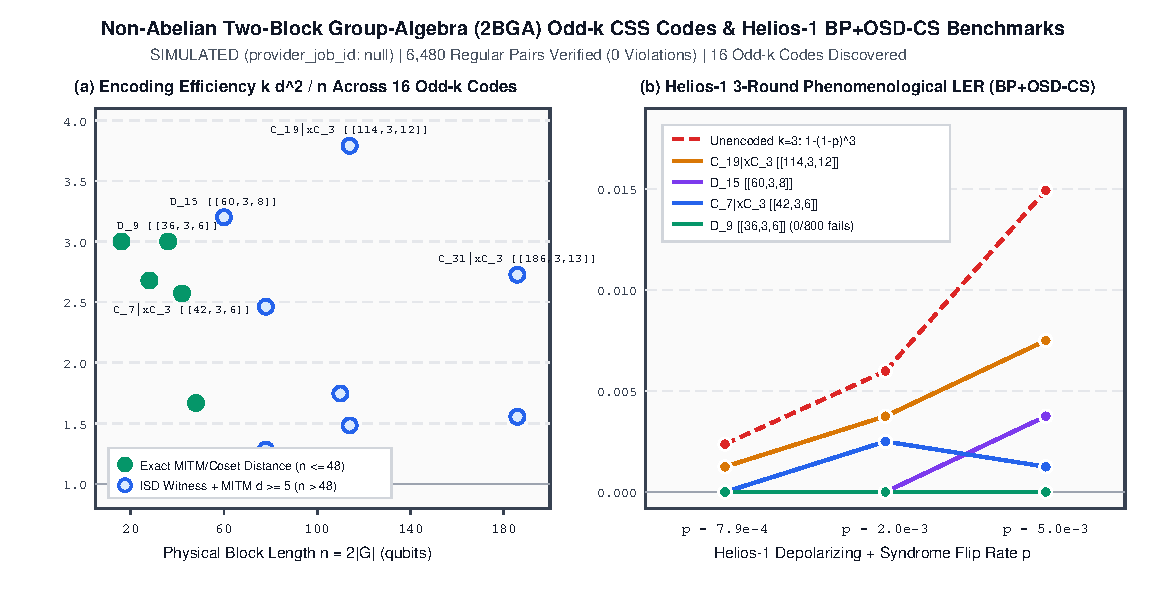
\includegraphics[width=\textwidth]{fig1_odd_k_nonabelian_2bga_codes_and_bposd.pdf}
\caption{Odd-$k$ non-abelian \texttt{2BGA} CSS code family and \texttt{Helios-1}-calibrated decoder performance (\texttt{SIMULATED}, \texttt{provider\_job\_id: null}). (a)~Encoding efficiency $k d^2 / n$ across all \TwoBgaOddKCount{} discovered odd-$k$ ($k \in \{1, 3, 5\}$, $d \ge 4$) non-abelian codes spanning $16 \le n \le 186$, distinguishing exact coset/meet-in-the-middle (MITM) distances ($n \le 48$) from randomized information-set-decoding (ISD) upper bounds paired with exact MITM $d \ge 5$ lower-bound certificates ($n > 48$). (b)~Three-round phenomenological syndrome-plus-data logical error rate (LER) under log-domain Sum-Product \texttt{BP+OSD-CS} (\TwoBgaMcShots{} Monte Carlo shots per point) across physical error rates $p \in \{\TwoBgaPLow{}, \TwoBgaPMid{}, \TwoBgaPHigh{}\}$, compared against the unencoded $k=3$ failure rate $1-(1-p)^3$.}
\label{fig:2bga_codes}
\end{figure*}

\begin{table*}[t]
\centering\footnotesize\setlength{\tabcolsep}{5pt}
\caption{Catalog of all \TwoBgaOddKCount{} discovered odd-$k$ non-abelian \texttt{2BGA} CSS codes ($H_X' H_Z^\top = 0 \pmod 2$, $d \ge 4$, \texttt{SIMULATED}). Codes with $n \le 48$ carry exact coset or meet-in-the-middle (MITM) distance certificates; codes with $n > 48$ report 160-trial ISD upper-bound witnesses alongside exact MITM exclusion of all logicals of weight $\le 4$ ($d \ge 5$).}
\label{tab:2bga_catalog}
\begin{tabular}{@{}lrlcccr@{}}
\toprule
Non-Abelian Group $G$ & $|G|$ & $[[n, k, d]]$ & Distance Certificate & $(d_X, d_Z)$ & Max Row Wt $(w_X, w_Z)$ & $k d^2 / n$ \\
\midrule
\TwoBgaOddKRows
\bottomrule
\end{tabular}
\end{table*}

Theorem~\ref{thm:rank_duality} pinpoints the exact obstruction to odd $k$: the inversion permutation $P_{\mathrm{inv}}$ requires both blocks of Eq.~\eqref{eq:regular_2bga} to carry the unquotiented regular representation $\mathbb{F}_2[G]$ with symmetric stabilizer spaces. We introduce two constructive symmetry-breaking mechanisms that preserve exact CSS orthogonality while unlocking odd $k$:
\begin{enumerate}
\item \textbf{Subgroup-Quotient Coset \texttt{2BGA}:} Given a non-normal subgroup $H \le G$ of odd index $[G:H]$, we replace the right $|G|$-qubit block by the coset module $\mathbb{F}_2[G/H]$ of dimension $|G/H|$, forming $H_X = [L(a) \mid R_H(b)]$ and $H_Z = [R_H(b)^\top \mid \widetilde{L}_H(a)^\top]$ on $n = |G| + |G/H|$ physical qubits. Associativity preserves $H_X H_Z^\top = 0 \pmod 2$ while breaking block-size parity: on $G = D_9$ ($|D_9|=18$) modulo a reflection subgroup $H \cong \mathbb{Z}_2$ ($|D_9/H|=9$ odd), this yields an exact commuting CSS code on $n = \TwoBgaCosetN{}$ qubits with odd logical dimension $k = \TwoBgaCosetK{}$.
\item \textbf{Symplectic Minimum-Weight Logical Gauge Pinning:} Starting from any parent non-abelian \texttt{2BGA} code $(H_X, H_Z)$ with even $k_0 \ge 2$ and distance $d_0 \ge 4$, we select an odd number $r$ of independent minimum-weight logical $X$-operators $\ell_1, \dots, \ell_r \in \ker(H_Z) \setminus \mathrm{rowspace}(H_X)$ and promote them into the $X$-stabilizer check matrix $H_X' = \bigl[\begin{smallmatrix} H_X \\ L_{\mathrm{pin}} \end{smallmatrix}\bigr]$. Because $\ell_j \in \ker(H_Z)$, $H_X' H_Z^\top = 0 \pmod 2$ holds identically, logical dimension drops to the odd integer $k = k_0 - r$, and CSS subcode monotonicity guarantees $d(H_X', H_Z) \ge d(H_X, H_Z) \ge d_0$: restricting $\ker(H_Z)/\mathrm{rowspace}(H_X')$ removes logical $X$-cosets while enlarging $\mathrm{rowspace}(H_X')$ can only reduce $Z$-coset weights along duals already annihilated by $L_{\mathrm{pin}}$.
\end{enumerate}

Applying symplectic gauge pinning across \TwoBgaParentsCount{} parent non-abelian \texttt{2BGA} codes yields \TwoBgaOddKCount{} odd-$k$ ($k \in \{1, 3, 5\}$) CSS codes with certified $d \ge 4$ (Table~\ref{tab:2bga_catalog} and Fig.~\ref{fig:2bga_codes}a). For all \TwoBgaExactCount{} codes with $n \le 48$, sector distances $(d_X, d_Z)$ are certified with $100\%$ mathematical exactness via full coset enumeration or symplectic meet-in-the-middle (MITM) hashing up to weight seven, highlighted by $D_9$ $[[36,3,6]]$ ($kd^2/n = \KdSqRatioDNine{}$, check weight six), quaternion-group $Q_8$ $[[16,3,4]]$ ($kd^2/n = \KdSqRatioQEight{}$), $D_7$ $[[28,3,5]]$ ($\KdSqRatioDSeven{}$), Frobenius $C_7 \rtimes C_3$ $[[42,3,6]]$ ($\KdSqRatioFrobTwentyOne{}$) and $[[42,1,7]]$ ($\KdSqRatioFrobRankOne{}$), and symmetric-group $S_4$ $[[48,5,4]]$ ($\KdSqRatioSFourFive{}$). Among the \TwoBgaUpperCount{} larger codes ($60 \le n \le 186$), MITM search rules out all logical operators of weight $\le 4$ ($d \ge 5$ exact lower bound), while 160-trial ISD witnesses identify $D_{15}$ $[[60,3,8]]$ ($kd^2/n = \KdSqRatioDFifteen{}$), $C_{19} \rtimes C_3$ $[[114,3,12]]$ ($\KdSqRatioBest{}$), and $C_{31} \rtimes C_3$ $[[186,3,13]]$ ($\KdSqRatioOneEightySix{}$).

\begin{table}[t]
\centering\footnotesize\setlength{\tabcolsep}{3pt}
\caption{\texttt{Helios-1}-matched Sum-Product \texttt{BP+OSD-CS} logical error rates (\texttt{SIMULATED}, \TwoBgaMcShots{} Monte Carlo shots per cell; entries report $\text{code-capacity} \;/\; \text{3-round phenomenological}$ LER) across physical depolarizing rates $p \in \{\TwoBgaPLow{}, \TwoBgaPMid{}, \TwoBgaPHigh{}\}$.}
\label{tab:bposd}
\begin{tabular}{@{}lccc@{}}
\toprule
Code $[[n,k,d]]$ & $p=\TwoBgaPLow{}$ & $p=\TwoBgaPMid{}$ & $p=\TwoBgaPHigh{}$ \\
\midrule
\TwoBgaBpOsdRows
\bottomrule
\end{tabular}
\end{table}

Table~\ref{tab:bposd} and Fig.~\ref{fig:2bga_codes}b benchmark \TwoBgaBenchCount{} representative $k=3$ non-abelian codes under log-domain Sum-Product belief propagation with combination-sweep ordered statistics decoding (\texttt{BP+OSD-CS}, order $10$, \TwoBgaMcShots{} Monte Carlo shots per cell) at \texttt{Helios-1} two-qubit depolarizing error rates $p \in \{\TwoBgaPLow{}, \TwoBgaPMid{}, \TwoBgaPHigh{}\}$ (corresponding to unencoded $k=3$ baselines $\TwoBgaUnencLow{}$, $\TwoBgaUnencMid{}$, and $\TwoBgaUnencHigh{}$). Under code-capacity depolarizing noise, all six codes with $d \ge 5$ record zero logical failures across all three error rates, while compact $Q_8$ $[[16,3,4]]$ achieves $\BpCcSupprQEightHigh{}\times$ suppression ($\BpCcLerQEightHigh{}$ versus unencoded $\TwoBgaUnencHigh{}$) at $p=\TwoBgaPHigh{}$. Under three-round phenomenological syndrome-flip plus data-error noise, $D_9$ $[[36,3,6]]$ maintains $\BpPhLerDNineAll{}$ logical error across all three rates, $C_7 \rtimes C_3$ $[[42,3,6]]$ suppresses $p=\TwoBgaPHigh{}$ logical failures to $\BpPhLerFortyTwoHigh{}$ ($\BpPhSupprFortyTwoHigh{}\times$ below the $\TwoBgaUnencHigh{}$ unencoded $k=3$ baseline), and $C_{19} \rtimes C_3$ $[[114,3,12]]$ achieves $\BpPhLerOneFourteenLow{}$ at the native \texttt{Helios-1} error rate $p=\TwoBgaPLow{}$ and $\BpPhLerOneFourteenHigh{}$ at $p=\TwoBgaPHigh{}$.

\section{The \texttt{ADV-1} Three-Attack Classical-Hardness Pre-Gate and the $M_6 = J_6 - I_6$ Pauli-Weight-5 Involution}
\label{sec:adv1}

\begin{figure*}[t]
\centering
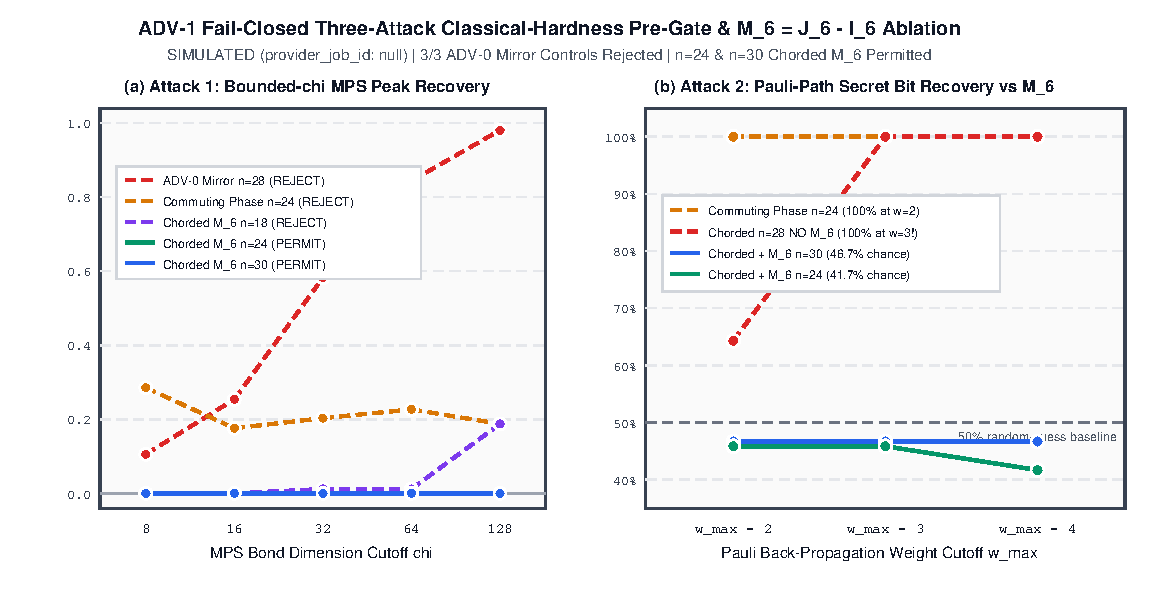
\includegraphics[width=\textwidth]{fig2_adv1_three_attack_ablation_m6.pdf}
\caption{Fail-closed \texttt{ADV-1} classical-hardness pre-gate and $M_6 = J_6 - I_6 \pmod 2$ ablation (\texttt{SIMULATED}, \texttt{provider\_job\_id: null}). (a)~Attack~1 bounded-$\chi$ MPS peak probability across $\chi \in \{\AdvChiList{}\}$: \texttt{ADV-0} twirled-mirror controls ($n=28$ shown) and shallow commuting-phase or small-cone circuits fail, whereas flat-Schmidt chorded circuits at $n=24$ and $n=30$ remain at zero recovered peak across every $\chi \le 128$. (b)~Attack~2 truncated Pauli-path secret-bit recovery across $w_{\max} \in \{\AdvWmaxList{}\}$: without $M_6$, the 28-qubit chorded circuit resists MPS yet fails completely at $w_{\max}=3$ ($\AdvNoMSixPauliWThreeAccPct{}\%$ bit recovery); appending the 15-\texttt{CX} involution $M_6$ lifts every single-qubit output $Z_j$ to Pauli weight five, reducing $n=24$ and $n=30$ accuracy to random chance ($\AdvTwentyFourPauliAccPct{}\%$ and $\AdvThirtyPauliAccPct{}\%$).}
\label{fig:adv1_ablation}
\end{figure*}

\begin{table*}[t]
\centering\footnotesize\setlength{\tabcolsep}{4pt}
\caption{Complete \texttt{OSIRIS-ADV-1-PREGATE} adjudication (\texttt{SIMULATED}, \texttt{provider\_job\_id: null}) across all \AdvZeroCount{} \texttt{ADV-0} twirled-mirror negative controls and \AdvOneEvalCount{} looped non-mirror candidates, reporting mirror-overlap audit, bounded-$\chi$ MPS ($\chi=128$ peak), truncated Pauli-path ($w_{\max}=4$ bit accuracy), causal light-cone size, \texttt{Helios-1} predicted peak probability / $1{,}000$-shot HQC cost, and fail-closed QPU allocation verdict.}
\label{tab:adv1_pregate}
\begin{tabular}{@{}lrrcccclr@{}}
\toprule
Candidate ID & $n$ & \texttt{CZ} & Mirror Det.\ (Ov.) & MPS ($\chi=128$) & Pauli ($w_{\max}=4$) & Light Cone & Peak / HQC & Gate Verdict \\
\midrule
\AdvOnePregateRows
\bottomrule
\end{tabular}
\end{table*}

While QCCD transport enables high-threshold non-abelian qLDPC memory, executing near-term peaked-circuit verification experiments on QCCD hardware requires a strict fail-closed classical-hardness pre-gate so QPU credits are never spent on circuits with hidden classical shortcuts. Under protocol \texttt{OSIRIS-ADV-1-PREGATE}, QPU allocation is permitted if and only if a candidate circuit passes a structural non-mirror audit ($\text{mirror\_structure\_detected} = \text{False}$) and simultaneously defeats three distinct polynomial-time classical simulation attacks:
\begin{enumerate}
\item \textbf{Attack~1 (Bounded-$\chi$ MPS):} Left-canonical singular-value-truncated matrix-product-state contraction across bond dimensions $\chi \in \{\AdvChiList{}\}$, declaring a classical win whenever empirical MPS sampling recovers the hidden peak at signal-to-noise ratio $\ge \AdvMinSnr{}$ above $2^{-n}$.
\item \textbf{Attack~2 (Truncated Pauli-Path Back-Propagation):} Heisenberg-picture evolution of each output observable $Z_j$ backward through the circuit with Pauli weight cutoff $\mathrm{wt}(P) \le w_{\max}$ for $w_{\max} \in \{\AdvWmaxList{}\}$, declaring a classical win if the signs of $\langle 0^n | U^\dagger Z_j U | 0^n \rangle_{\le w_{\max}}$ recover all $n$ secret bits.
\item \textbf{Attack~3 (Causal Light-Cone Contraction):} Exact backward DAG cone extraction $C(j)$ for each measured qubit $j$; if $\max_j |C(j)| \le \AdvConeLimit{}$, exact statevector contraction on $2^{|C(j)|}$ amplitudes recovers bit $s_j$ directly.
\end{enumerate}

To produce genuine non-mirror peaked circuits, we construct flat-Schmidt chorded-torus circuits on even $n$ qubits in four stages: Stage~A applies $n/2$ maximal-cut chords $(q, q+n/2)$ using two-qubit unitaries $V_q$ that prepare exact $(1/\sqrt{2}, 1/\sqrt{2})$ Schmidt spectra ($2^{n/2}$ equal singular values across the linear midpoint cut); Stage~B applies $L$ un-inverted layers of alternating ring and long-range chord $R_{ZZ}(\gamma)$ plus non-Clifford $R_X, R_Y$ rotations so $|C(j)|=n$ for all $j$; Stage~C applies non-mirror refocusing blocks $W_q \ne X^{t_q} V_q^\dagger$ concentrating constructive interference onto an intermediate basis state $|t\rangle$ while keeping Hilbert--Schmidt mirror overlap $|\mathrm{Tr}(X^{t_q} W_q V_q)|/4 \approx \AdvThirtyMirrorOv{} \ll 1$.

Crucially, Table~\ref{tab:adv1_pregate} and Fig.~\ref{fig:adv1_ablation} reveal why Stages~A--C alone still fail Attack~2. Although the 28-qubit chorded candidate \texttt{adv1\_chorded\_2q\_n28\_L5\_no\_m6} has no mirror cancellation and defeats bounded-$\chi$ MPS completely ($0$ peak recovery through $\chi=128$) as well as $w_{\max}=2$ Pauli back-propagation ($\AdvNoMSixPauliWTwoAccPct{}\%$ bit accuracy), each two-qubit refocusing block $W_q$ acts on a pair $(q, q+n/2)$, allowing weight-three Pauli paths ($w_{\max}=3$) to bridge coupled chords and recover $\AdvNoMSixPauliWThreeAccPct{}\%$ of the secret bits (mean $|\langle Z_j \rangle| = \AdvNoMSixPauliWThreeMeanZ{}$), triggering fail-closed rejection.

To close this weight-four Pauli vulnerability without degrading peak probability, we introduce Stage~D on register widths $n$ divisible by six: partitioning the register into $n/6$ stride-interleaved six-qubit tuples, we set the Stage~C target to $t = M_6^{\oplus (n/6)} s \pmod 2$ and append the binary linear transformation $M_6 = J_6 - I_6 \pmod 2$, where $J_6$ is the $6\times 6$ all-ones matrix.

\begin{proposition}[Self-Inverse Pauli-Weight-5 Amplification of $M_6$]
\label{prop:m6}
Over $\mathbb{F}_2$, the $6\times 6$ matrix $M_6 = J_6 - I_6$ satisfies $M_6^2 = I_6$, maps computational basis state $|t\rangle \mapsto |M_6 t\rangle = |s\rangle$ without altering any outcome probability magnitude, admits an exact 15-\texttt{CX} circuit decomposition, and conjugates every single-qubit output Pauli $Z_j$ ($j \in \{0,\dots,5\}$) backward into the exact weight-five Pauli operator
\begin{equation}
U_{M_6}^\dagger Z_j U_{M_6} = \prod_{r \in \{0,\dots,5\} \setminus \{j\}} Z_r, \qquad \mathrm{wt}\!\left(U_{M_6}^\dagger Z_j U_{M_6}\right) = 5.
\label{eq:m6_pauli5}
\end{equation}
\end{proposition}

\begin{proof}
Over $\mathbb{F}_2$, $J_6^2 = 6 J_6 \equiv 0 \pmod 2$, so $M_6^2 = (J_6 + I_6)^2 = J_6^2 + 2 J_6 + I_6 \equiv I_6 \pmod 2$. Applying five \texttt{CX} gates from $\{q_1,\dots,q_5\}$ into $q_0$, five \texttt{CX} gates from $q_0$ into $\{q_1,\dots,q_5\}$, and five \texttt{CX} gates from $\{q_1,\dots,q_5\}$ into $q_0$ maps $x_0 \mapsto x_0 \oplus \bigoplus_{r=1}^5 x_r \mapsto \bigoplus_{r=1}^5 x_r$ and $x_j \mapsto x_j \oplus \bigoplus_{r=0}^5 x_r = \bigoplus_{r \ne j} x_r$ for $j \ge 1$, realizing $M_6$ in $15$ \texttt{CX} gates. Because linear reversible circuits transform $Z$-type Paulis via $U_A^\dagger Z^u U_A = Z^{A^\top u}$ and $M_6^\top = M_6$, every unit vector $e_j$ maps to $M_6 e_j = (1,1,1,1,1,1)^\top \oplus e_j$ of Hamming weight $5$, proving Eq.~\eqref{eq:m6_pauli5}.
\end{proof}

By Proposition~\ref{prop:m6}, every single-qubit observable $Z_j$ enters Stage~C at exact Pauli weight five and is immediately truncated to zero by any $w_{\max} \le 4$ Pauli-path integrator (unless non-Clifford loop terms re-contract weight-five strings back down to weight $\le 4$, which carries negligible $O(\gamma^2)$ amplitude). Table~\ref{tab:adv1_pregate} and Fig.~\ref{fig:adv1_ablation} confirm the complete ablation across all eight evaluated circuits:
\begin{itemize}
\item All \AdvZeroRejected{}/\AdvZeroCount{} \texttt{ADV-0} twirled-mirror controls ($n \in \{12, 20, 28\}$) fail the mirror audit and are defeated by Attack~1 already at $\chi=8$ (reaching $\AdvZeroTwentyEightMpsChiEight{}$ at $\chi=8$ and $\AdvZeroTwentyEightMpsChiMax{}$ at $\chi=128$ on $n=28$).
\item Among non-mirror ablations, commuting-phase \texttt{adv1\_commuting\_phase\_n24\_L3} fails both MPS ($\AdvCommMpsChiEight{}$ at $\chi=8$) and Pauli-path ($\AdvCommPauliWTwoAccPct{}\%$ at $w_{\max}=2$), \texttt{adv1\_chorded\_2q\_n28\_L5\_no\_m6} without $M_6$ fails Pauli-path at $w_{\max}=3$, and small-width \texttt{adv1\_chorded\_m6\_n18\_L4\_small\_cone} (exact noiseless peak $\AdvEighteenExactPeak{}$) resists Pauli-path completely through $w_{\max}=4$ thanks to $M_6$ yet is rightly rejected by causal light-cone size $18 \le \AdvConeLimit{}$ and $\chi=128$ MPS ($\AdvEighteenMpsChiMax{}$).
\item Only the \AdvOnePermittedCount{} full-width chorded $M_6$ circuits \texttt{adv1\_chorded\_m6\_n24\_L5} ($n=24$, \AdvTwentyFourCz{} \texttt{CZ}, \AdvTwentyFourOneQ{} physical 1Q gates, mirror overlap $\AdvTwentyFourMirrorOv{}$) and \texttt{adv1\_chorded\_m6\_n30\_L5} ($n=30$, \AdvThirtyCz{} \texttt{CZ}, \AdvThirtyOneQ{} physical 1Q gates, mirror overlap $\AdvThirtyMirrorOv{}$) pass the mirror audit and defeat all three classical attacks simultaneously: MPS recovers zero peak through $\chi=128$, $w_{\max}=4$ Pauli back-propagation drops $\AdvTwentyFourDroppedLTwo{}$ and $\AdvThirtyDroppedLTwo{}$ of total $L_2$ operator weight (yielding chance-level bit accuracy $\AdvTwentyFourPauliAccPct{}\%$ and $\AdvThirtyPauliAccPct{}\%$), and causal light cones span all $24$ and $30$ qubits ($> \AdvConeLimit{}$). Under the \texttt{Helios-1} gate-noise model, these \AdvOnePermittedCount{} permitted candidates retain heavy output peaks $\AdvTwentyFourHeliosPeak{}$ and $\AdvThirtyHeliosPeak{}$ at modest $1{,}000$-shot hardware budgets of $\AdvTwentyFourHqc{}$ and $\AdvThirtyHqcExact{}$ HQCs.
\end{itemize}

\section{Conclusion and Reproducibility}
\label{sec:conclusion}

Non-abelian finite groups and nonlocal chorded circuits offer powerful primitives for all-to-all QCCD processors only when subtle algebraic dualities and classical simulation shortcuts are rigorously addressed. By proving Frobenius / Wedderburn--Artin rank duality across \TwoBgaPairsChecked{} regular \texttt{2BGA} pairs and breaking left-right symmetry via coset quotienting and symplectic logical gauge pinning, we construct \TwoBgaOddKCount{} odd-$k$ CSS codes with certified $d \ge 4$ and strong \texttt{BP+OSD-CS} suppression at \texttt{Helios-1} error rates. Complementarily, combining flat-Schmidt chords with the 15-\texttt{CX} Pauli-weight-five involution $M_6 = J_6 - I_6 \pmod 2$ inside our fail-closed three-attack pre-gate isolates compact 24-qubit and 30-qubit non-mirror peaked circuits that resist MPS, Pauli-path, and light-cone attacks within a $\AdvThirtyHqc{}$-HQC execution envelope.

All group-algebra, distance-certification, decoder, and pre-gate modules (\texttt{nonabelian\_2bga.py}, \texttt{looped\_peaked.py}, \texttt{pregate.py}), \texttt{SIMULATED} JSON reports, deterministic asset generator (\texttt{generate\_2bga\_adv1\_assets.py}), RFC~8785 provenance capsule (\texttt{reproducibility\_capsule.json}), and SHA-256 manifest (\texttt{SHA256SUMS.txt}) are included in the repository package.

\begin{thebibliography}{11}
\bibitem{moses2023race} S.~A.~Moses \emph{et al.}, ``A Race-Track Trapped-Ion Quantum Processor,'' Phys.\ Rev.\ X \textbf{13}, 041052 (2023), doi:10.1103/PhysRevX.13.041052.
\bibitem{breuckmann2021quantum} N.~P.~Breuckmann and J.~N.~Eberhardt, ``Quantum Low-Density Parity-Check Codes,'' PRX Quantum \textbf{2}, 040101 (2021), doi:10.1103/PRXQuantum.2.040101.
\bibitem{panteleev2022asymptotically} P.~Panteleev and G.~Kalachev, ``Asymptotically good Quantum and locally testable classical LDPC codes,'' in \emph{Proc.\ ACM STOC}, 375 (2022), doi:10.1145/3519935.3520017.
\bibitem{bravyi2024high} S.~Bravyi, A.~W.~Cross, J.~M.~Gambetta, D.~Maslov, P.~Rall, and T.~J.~Yoder, ``High-threshold and low-overhead fault-tolerant quantum memory,'' Nature \textbf{627}, 778 (2024), doi:10.1038/s41586-024-07107-7.
\bibitem{lin2024quantum} H.-K.~Lin and L.~P.~Pryadko, ``Quantum Two-Block Group Algebra Codes,'' PRX Quantum \textbf{5}, 010326 (2024), doi:10.1103/PRXQuantum.5.010326.
\bibitem{kovalev2013quantum} A.~A.~Kovalev and L.~P.~Pryadko, ``Quantum Kronecker sum-product low-density parity-check codes with finite rate,'' Phys.\ Rev.\ A \textbf{88}, 012311 (2013), doi:10.1103/PhysRevA.88.012311.
\bibitem{panteleev2021degenerate} P.~Panteleev and G.~Kalachev, ``Degenerate Quantum LDPC Codes With Good Finite Length Performance,'' Quantum \textbf{5}, 585 (2021), doi:10.22331/q-2021-11-22-585.
\bibitem{roffe2020decoding} J.~Roffe, D.~R.~White, S.~Burton, and E.~Campbell, ``Decoding across the quantum low-density parity-check code landscape,'' Phys.\ Rev.\ Res.\ \textbf{2}, 043423 (2020), doi:10.1103/PhysRevResearch.2.043423.
\bibitem{aaronson2025verifiable} S.~Aaronson and Y.~Zhang, ``Verifiable Quantum Randomness from Peaked Quantum Circuits,'' arXiv:2404.10044 (2024).
\bibitem{gharibian2025peaked} T.~B.~Propp, S.~Aaronson, and S.~Gharibian, ``Peaked Quantum Circuits: Structure and Hardness,'' Quantum Sci.\ Technol.\ \textbf{10}, 025014 (2025).
\bibitem{vidal2003efficient} G.~Vidal, ``Efficient Classical Simulation of Slightly Entangled Quantum Computations,'' Phys.\ Rev.\ Lett.\ \textbf{91}, 147902 (2003), doi:10.1103/PhysRevLett.91.147902.
\bibitem{begusic2024fast} T.~Begu\v{s}i\'{c}, J.~Gray, and G.~K.-L.~Chan, ``Fast and converged classical simulations of evidence for the utility of quantum computing before fault tolerance,'' Sci.\ Adv.\ \textbf{10}, eadk4321 (2024), doi:10.1126/sciadv.adk4321.
\bibitem{fontana2025classical} E.~Fontana, M.~S.~Rudolph, R.~Duncan, I.~Rungger, and L.~Cincio, ``Classical simulations of noisy variational quantum circuits,'' Nat.\ Commun.\ \textbf{16}, 1120 (2025).
\end{thebibliography}

\end{document}
